\documentclass{jhwhw}
%\everymath{\displaystyle}
\usepackage{color}
%\usepackage{bm}
\usepackage{amsmath}
%\usepackage{setspace}
%\usepackage{verbatim}
\usepackage{graphicx}
%\usepackage[lmargin=2.5cm, rmargin=2.5cm,tmargin=3cm,bmargin=2.5cm]{geometry}
\usepackage{hyperref}
\hypersetup{
colorlinks=true,
linkcolor=blue,
urlcolor=blue
}

\def\@Aboxed#1&#2\ENDDNE{%
  \settowidth\@tempdima{$\displaystyle#1{}$}%
  \addtolength\@tempdima{\fboxsep}%
  \addtolength\@tempdima{\fboxrule}%
  \global\@tempdima=\@tempdima
  \kern\@tempdima
  &
  \kern-\@tempdima
  \fcolorbox{red}{yellow}{$\displaystyle #1#2$}
}

\author{Bret Comnes}
\title{QM Homework 2}

\begin{document}
\problem{Scattering by a 3D atractive spherical well}
	Consider scattering by the following 3D attractive spherical potential well:
	\begin{equation}
		\label{eq:swell}
		V(r) =
		\begin{cases}
			-V_0, & 0 < r < a\\
			0, & a < r
		\end{cases}
	\end{equation}
	See the main homework problem statement for more information, but for reference, the importaint equasions from the problem statement are the following:
	\begin{equation}
		\label{eq:alpha}
		\alpha^2 \equiv k^2 + \frac{2 m}{\hbar^2}V_0
	\end{equation}
	General non-singular solutions to the potential.
	\begin{equation}
		\label{eq:rl}
		R_l = 
		\begin{cases}
			A_l j_l(\alpha r) \\
			B_l j_l(k r) + C_l n_l(k r)
		\end{cases}
	\end{equation}
\part
	Show that the logarithmic deritiative which must be matched at r = a can be expressed as:
	\begin{equation}
		\label{eq:1aderiv}
		\frac{1}{R_l}\frac{dR_l}{dr}|_{r=a_-}\equiv \frac {1} {a \gamma_l (k)}
	\end{equation}
	where
	\begin{equation}
		\label{eq:gammal}
		\gamma_l (k) = \frac {j_l(\alpha a)} {\alpha a j'_l(\alpha a)}
	\end{equation}
\solution

Let's start with plugging in $R_l$ into Equation~\eqref{eq:1aderiv}, taking into account that it wants us to be to the left of the boundary condition, and evaluate at $r = a$ after the derivative.  	

\begin{align}
	\frac{1}{R_l}\frac{dR_l}{dr}|_{r=a_-} &= \frac{1}{A_l j_l(\alpha r) }\frac{d}{dr}|_{r=a_-}A_l j_l(\alpha r)
	\\  &= \frac{1}{ j_l(\alpha r) } \frac {A_l}{A_l} \frac{d}{dr} j_l(\alpha r) |_{r=a_-}
	\\  &= \frac{1}{ j_l(\alpha r) } j'_l(\alpha r) \frac{d}{dr} \alpha r |_{r=a_-}
	\\  &= \frac{1}{ j_l(\alpha r) }  \alpha j'_l(\alpha r)|_{r=a_-}
	\\  &= \frac{\alpha j'_l(\alpha a)}{ j_l(\alpha a) }
\end{align}

Multiplying by $1 = \frac{a}{a}$ and substituting in in $\gamma_l$ we get

\begin{align}
	\Aboxed{\frac{a}{a}\frac{\alpha j'_l(\alpha a)}{ j_l(\alpha a) } &= \frac{1}{a \gamma_l(k)}}
\end{align}

\part
	Find an \underline{exact} expression for the phase shift $\delta_l$ using the result for the $\tan(\delta_l)$ given by 

\begin{align}
    \label{eq:tandl1}
	\tan \delta_l = \frac {k a \gamma_l (k) j'_l(k a)-j_l (k a)}{k a \gamma_l(k)\eta'_l(ka)-\eta_l(ka)}
\end{align}
or Eq. 15.2 in the notes.  

\solution
Lets start by subbing in Equation~\eqref{eq:gammal} into \eqref{eq:tandl1}.

\begin{align}
	\tan \delta_l &= \frac {k a \frac {j_l(\alpha a)} {\alpha a j'_l(\alpha a)} j'_l(k a)-j_l (k a)}{k a \frac {j_l(\alpha a)} {\alpha a j'_l(\alpha a)}\eta'_l(ka)-\eta_l(ka)}
	\\ &= \frac {k a \frac {j_l(\alpha a)} {\alpha a j'_l(\alpha a)} j'_l(k a)-j_l (k a)}{k a \frac {j_l(\alpha a)} {\alpha a j'_l(\alpha a)}\eta'_l(ka)-\eta_l(ka)} \frac {\alpha a j'_l(\alpha a)}{\alpha a j'_l(\alpha a)}
	\\ &= \frac {k j_l(\alpha a) j'_l(k a)- \alpha j'_l(\alpha a) j_l (k a)}{k j_l(\alpha a) \eta'_l(ka)-\alpha j'_l(\alpha a) \eta_l(ka)}
	\label{eq:tand1}
	\\ \Aboxed{\delta_l &= \tan^{-1}{\left( \frac {k j_l(\alpha a) j'_l(k a)- \alpha j'_l(\alpha a) j_l (k a)}{k j_l(\alpha a) \eta'_l(ka)-\alpha j'_l(\alpha a) \eta_l(ka)}\right)}}
\end{align}
\pagebreak[4]

\part
Show that the s-wave phase shift is given by
\begin{equation}
	\delta_0 = -k a + \tan^{-1}\left[{\frac{k}{\alpha} \tan{(\alpha a)}}\right]
\end{equation}
where
\begin{align}
	j_0(x) &= \frac{\sin{x}}{x} & 
	\eta_0(x)= - \frac{cos{x}}{x}
\end{align}

\solution
Starting with Equation~\eqref{eq:tand1}, we want to begin to sub in what we know for $j_0$ and $\eta_0$, but first we need to know their derivatives.

\begin{align}
	\label{eq:j0}
	j_0(\alpha a) &= \frac{\sin{\alpha a}}{\alpha a} & 
	\eta_0(\alpha a)&= - \frac{\cos{\alpha a}}{\alpha a}
	 \\\label{eq:j0p}
	j'_0(\alpha a) &= \frac {\alpha^2 a \cos{(\alpha a)} - \alpha \sin{(\alpha a)}} {\alpha^2 a^2} & 
	\eta'_0(\alpha a) &= \frac {\alpha^2 a \sin{(\alpha a)} + \alpha \cos{(\alpha a)}} {\alpha^2 a^2}
\end{align}

It also I managed to do the algebra using the following substitutions:
\begin{align}
	\label{eq:absub}
	A &= \alpha a & B &= k a
\end{align}

With all this in mind we can now sub in Equation~\eqref{eq:j0},~\eqref{eq:j0p} and \eqref{eq:absub} into Equation~\eqref{eq:tand1}

\begin{align}
    \tan{\delta_0} &= 
	\frac 
	{k \frac{\sin{\alpha a}}{\alpha a} \frac {k^2 a \cos{(k a)} - k \sin{(k a)}} {k^2 a^2} - \alpha \frac {\alpha^2 a \cos{(\alpha a)} - \alpha \sin{(\alpha a)}} {\alpha^2 a^2} \frac{\sin{k a}}{k a}}
	{k \frac{\sin{\alpha a}}{\alpha a} \frac {k^2 a \sin{(k a)} + k \cos{(k a)}} {k^2 a^2}+\alpha \frac {\alpha^2 a \cos{(\alpha a)} - \alpha \sin{(\alpha a)}} {\alpha^2 a^2}\frac{\cos{ka}}{k a}} 
	\\
	&= \frac
	{k \frac{\sin{A}}{A} \frac {k^2 a \cos{(B)} - k \sin{(B)}} {B^2} - \alpha \frac {\alpha^2 a \cos{(A)} - \alpha \sin{(A)}} {A^2} \frac{\sin{B}}{B}}
	{k \frac{\sin{A}}{A} \frac {k^2 a \sin{(B)} + k \cos{(B)}} {B^2}+\alpha \frac {\alpha^2 a \cos{(A)} - \alpha \sin{(A)}} {A^2}\frac{\cos{B}}{B}} \frac{A^2 B^2}{A^2 B^2} 
	\\
	&= \frac
	{
	A(k^3 a \sin{A}\cos{B}- k^2 \sin{A}\sin{b})-B(\alpha^3 a \sin{B}\cos{A}-\alpha^2 \sin{A}\sin{B})
	}
	{
	A(k^3 a \sin{A}\sin{B}+k^2 \sin{A} \cos{B} + B(\alpha^3 a \sin{B}\cos{A}-\alpha^2 \sin{A}\sin{B})
	}\frac{a^2}{a^2}
	\\
	&= \frac
	{
	A(B^3 \sin{A}\cos{B}- B^2 \sin{A}\sin{b})-B(A^3 \sin{B}\cos{A}- A^2 \sin{A}\sin{B})
	}
	{
	A(B^3  \sin{A}\sin{B}+B^2 \sin{A} \cos{B} + B(A^3 \sin{B}\cos{A}-A^2 \sin{A}\sin{B})
	} \frac{(AB)^{-1}}{(AB)^{-1}}
	\\
	&= \frac
	{
	B^2 \sin{A}\cos{B}- B \sin{A}\sin{b} - A^2 \sin{B}\cos{A}- A \sin{A}\sin{B}
	}
	{
	B^2  \sin{A}\sin{B}+B \sin{A} \cos{B} + A^2 \sin{B}\cos{A}-A \sin{A}\sin{B}
	}
	\\
	&= \frac 
	{
	B^2 \sin{A} \left( \frac{\cos{B}}{B} - \frac {\sin{B}}{B^2} \right) - A^2 \sin{B} \left( \frac { \cos{A} } { A } - \frac {  \sin{A}  } {  A^2  } \right)
	}
	{
	B^2 \sin{A} \left( \frac{\cos{B}}{B^2} + \frac {\sin{B}}{B} \right) + A^2 \cos{B} \left( \frac { \cos{A} } { A } - \frac {  \sin{A}  } {  A^2  } \right)
	}
\end{align}

Lets call
\begin{align}
	g &=  \left( \frac { \cos{A} } { A } - \frac {  \sin{A}  } {  A^2  } \right) & f &= \left( \frac{\cos{B}}{B} - \frac {\sin{B}}{B^2} \right) & h &= \left( \frac{\cos{B}}{B} + \frac {\sin{B}}{B^2} \right)
\end{align}
so that we can do a whole lot more of algebra.
\begin{align}
	\tan{\delta_0} &= \frac 
	{
	B^2 \sin{(A)} f - A^2 \sin{(B)} g
	}
	{
	B^2 \sin{(A)} h + A^2 \cos{(B)} g
	} 
	\\
	&= \left(\frac{\sin{B}}{\cos{B}}\right) \frac 
	{
	B^2 \sin{(A)} f \frac{1}{\sin{B}} - A^2 g
	}
	{
	B^2 \sin{(A)} h \frac{1}{\cos{B}} + A^2 g
	}
	\\
	&= \left(\tan{B}\right) \frac 
	{
	B^2 \sin{(A)} \left( \frac{\cos{B}}{B} - \frac {\sin{B}}{B^2} \right) \frac{1}{\sin{B}} - A^2 g
	}
	{
	B^2 \sin{(A)} \left( \frac{\cos{B}}{B} + \frac {\sin{B}}{B^2} \right) \frac{1}{\cos{B}} + A^2 g
	}
	\\	
	&= \left(\tan{B}\right) \frac 
	{
	B^2 \sin{(A)} \left( \frac{\cos{B}}{B \sin{B}} - \frac {\sin{B}}{B^2 \sin{B}} \right) - A^2 g
	}
	{
	B^2 \sin{(A)} \left( \frac{\cos{B}}{B^2 \cos{B}} + \frac {\sin{B}}{B \cos{B}} \right) + A^2 g
	}
	\\
	&= \left(\tan{B}\right) \frac 
	{
	B^2 \sin{(A)} \left( \frac{\cot{B}}{B} - \frac {1}{B^2} \right) - A^2 \left( \frac { \cos{A} } { A } - \frac {  \sin{A}  } {  A^2  } \right)
	}
	{
	B^2 \sin{(A)} \left(\frac {\tan{B}}{B} + \frac{1}{B^2} \right) + A^2 \left( \frac { \cos{A} } { A } - \frac {  \sin{A}  } {  A^2  } \right)
	}
	\\
	&= \left(\tan{B}\right) \left(\frac{\sin{A}}{\sin{A}}\right) \frac 
	{
	B^2 \left( \frac{\cot{B}}{B} - \frac {1}{B^2} \right) - A^2 \left( \frac { \cos{A} } { A \sin{A} } - \frac {  \sin{A}  } {  A^2 \sin{A}  } \right)
	}
	{
	B^2	\left(\frac {\tan{B}}{B} + \frac{1}{B^2} \right) + A^2 \left( \frac { \cos{A} } { A \sin{A} } - \frac {  \sin{A}  } {  A^2 \sin{A} } \right)
	}
	\\
	&= \left(\tan{B}\right) \frac 
	{
	\left( B \cot{B} - 1 \right) - A^2 \left( \frac { \cos{A} } { A \sin{A} } - \frac {  \sin{A}  } {  A^2 \sin{A}  } \right)
	}
	{
	\left( B \tan{B} - 1 \right) + A^2 \left( \frac { \cos{A} } { A \sin{A} } - \frac {  \sin{A}  } {  A^2 \sin{A} } \right)
	}
	\\
	&= \left(\tan{B}\right) \frac 
	{
	B \cot{B} - 1 - A \cot{A}+1
	}
	{
	B \tan{B} - 1 + A \cot{A} - 1
	}
	\\
	&= \frac 
	{
	B - A \cot{A}\tan{B}
	}
	{
	B \tan{B} + A \cot{A}
	} \frac{\tan{A}}{\tan{A}}
	\\
	&= \frac 
	{
	B \tan{A} - A \tan{B}
	}
	{
	B \tan{B}\tan{A} + A 
	}
	\\
	&= \frac 
	{
	\frac{B}{A} \tan{A} - \tan{B}
	}
	{
	\frac{B}{A} \tan{B}\tan{A} + 1 
	}
	\\
	\label{eq:tandelta2}
	&= \frac 
	{
	\frac{k}{\alpha} \tan{\alpha a} - \tan{k a}
	}
	{
	\frac{k}{\alpha} \tan{k a}\tan{\alpha a} + 1 
	}
\end{align}
Remembering that
\begin{align}
    \tan{(\tan^{-1}{(x)})}=x
\end{align}
and that 
\begin{align}
    \tan{(X - Y)} = \frac{\tan{X}-\tan{Y}}{1+\tan{X}\tan{Y}}
\end{align}
we can consider the following
\begin{align}
    X &= \tan^{-1}{\left( \frac{B}{A} \tan{A}\right)} & Y & = \tan{B}
\end{align}
so that
\begin{align}
    \tan{\delta_0} &= \frac 
	{
	\tan{\left(\tan^{-1}{\left(\frac{B}{A} \tan{A}\right)}\right)} - \tan{B}
	}
	{
	1 + \tan{\left(\tan^{-1}{\left(\frac{B}{A} \tan{A}\right)}\right)}\tan{B} 
	} 
	\\
	&= \tan{\left( \tan^{-1}{\left( \frac{B}{A} \tan{A}\right)} - B \right)}
\end{align}
and finally getting rid of the $\tan$ function around $\delta_0$, and putting back $A$ and $B$
\begin{align}
    \tan^{-1}{(\tan{\delta_0})} &= \tan^{-1}{\left(\tan{\left( \tan^{-1}{\left( \frac{B}{A} \tan{A}\right)} - B \right)}  \right)}
    \\
    \delta_0 &= \tan^{-1}{\left( \frac{B}{A} \tan{A}\right)} - B
    \\
    \label{eq:delta0}
    \Aboxed{\delta_0 &= - k a + \tan^{-1}{\left[ \frac{k}{\alpha} \tan{\alpha a}\right]}} 
\end{align}
\pagebreak[4]

\part
Show that the \underline{scattering length} for s-wave scattering is given by:
\begin{equation}
    \label{eq:L}
    L = -\lim_{x \to 0} \frac{\tan{\delta_0}}{k} = a - \frac{(\tan{\lambda a})}{\lambda}
\end{equation}
where
\begin{equation}
    \lambda = \sqrt{\frac{2m}{\hbar^2}V_0}
\end{equation}
\solution
Lets start taking the limit of \eqref{eq:L} with \eqref{eq:delta0} plugged in.
\begin{align}
    L = -\lim_{k \to 0} \frac{\tan{\left(   - k a + \tan^{-1}{\left[ \frac{k}{\alpha} \tan{\alpha a}\right]}   \right)}}{k}
\end{align}

With some simple investigation, we see that we are coming across a limit of an indefinite form.
\begin{equation}
    L = -\lim_{k \to 0} \frac{0}{0}
\end{equation}  
Lets use L'Hopital's rule:
\begin{equation}
    \mathop {\lim }\limits_{x \to c} \frac{{f\left( x \right)}}{{g\left( x \right)}} = \mathop {\lim }\limits_{x \to c} \frac{{f'\left( x \right)}}{{g'\left( x \right)}}
\end{equation}
Taking the derivative of $f(x)$ will require the quotient rule:
\begin{equation}
    \frac{d}{dk}\left[\frac{f(k)}{g(k)}\right]=\frac{   f'(k)g(k) - f(k)g'(k)    }{g(k)^2}
\end{equation}
Lets start with each derivative individually, using the form of $\tan{\delta_0}$ in Equation~\eqref{eq:tandelta2}.
\begin{align}
    f(k) &= \frac{k}{\alpha} \tan{\alpha a} - \tan{k a} & g(k) &= \frac{k}{\alpha} \tan{k a}\tan{\alpha a} + 1  \\ 
    f'(k) &= \frac{1}{\alpha}\tan{(\alpha a)} - a \sec^{2}{(a k)} & g'(k) &=  k \sec^{2}{(a k)}\tan{(\alpha a)}+\frac{\tan{(a k)}\tan{(\alpha a)}}{a} \\
    & & f(k)^2 &= \left( \frac{k}{\alpha} \tan{k a}\tan{\alpha a} + 1 \right)^2
\end{align}
Putting it all together now:
\begin{align}
    \lim_{k \to 0}g(k)f'(k) &= \lim_{k \to 0}\left( \frac{1}{\alpha}\tan{(\alpha a)} - a \sec^{2}{(a k)} \right) \lim_{k \to 0}\left( \frac{k}{\alpha} \tan{k a}\tan{\alpha a} + 1 \right) \\
    &= \left( \frac{1}{\alpha}\tan{(\alpha a)} - a \right)(1) = \frac{1}{\alpha}\tan{(\alpha a)} - a\\
    \lim_{k \to 0}f(k)g'(k) &= \lim_{k \to 0} \left( \frac{k}{\alpha} \tan{\alpha a} - \tan{k a} \right) \lim_{k \to 0} \left( k \sec^{2}{(a k)}\tan{(\alpha a)}+\frac{\tan{(a k)}\tan{(\alpha a)}}{a} \right)\\
    &= 0 \\
    \lim_{k \to 0}g(k)^2  &= \left(\lim_{k \to 0} \left( \frac{k}{\alpha} \tan{k a}\tan{\alpha a} + 1 \right) \right)^2 \\
    & = 1 \\
    \lim_{x \to 0} \frac{\tan{\delta_0}}{k} &= \frac {\frac{\left(\frac{1}{\alpha}\tan{(\alpha a)} - a\right) - 0} {1}}{1} \\
    &= \frac{1}{\alpha}\tan{(\alpha a)} - a
\end{align}

Plugging in for $\alpha$ where
\begin{equation}
    \alpha^2 = k^2 + \frac{2m}{\hbar^2}V_0
\end{equation}
and taking $k \to 0$ and plugging in $\lambda$, we get 
\begin{align}
    L = -\lim_{x \to 0} \frac{\tan{\delta_0}}{k} &= -\frac{1}{\sqrt{\frac{2m}{\hbar^2}V_0}}\tan{\left(\sqrt{\frac{2m}{\hbar^2}V_0} a\right)} + a \\
   \Aboxed{L &= a - \frac{(\tan{\lambda a})}{\lambda}} \label{eq:Lfinal}
\end{align}
\pagebreak[4]

\part
Discuss the dependance of $L$ on the potential strength $(\lambda)$ and the potential range $a$.
\solution
\begin{figure}[htbp]
    \centering
        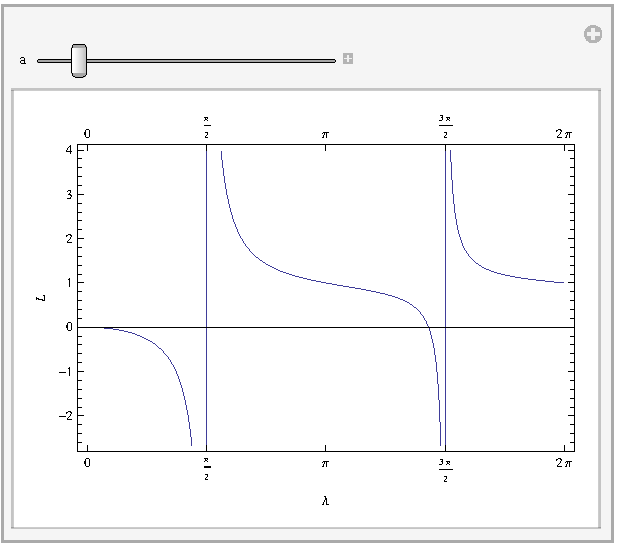
\includegraphics[height=2.8in]{LofLambda.pdf} 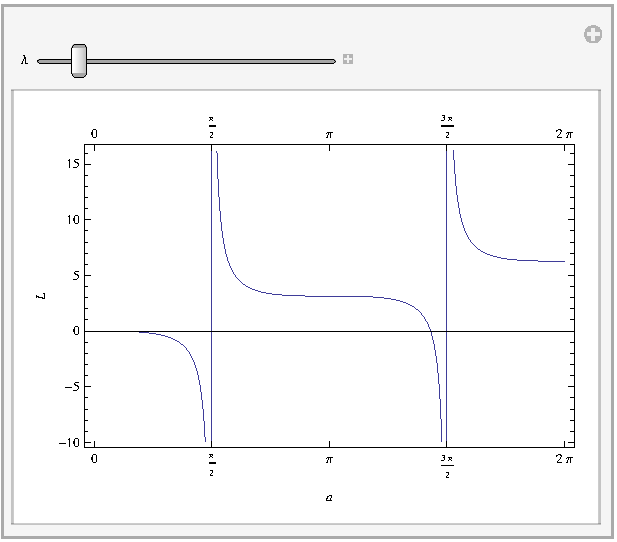
\includegraphics[height=2.8in]{Lofa.pdf}
    \caption{Plots of $L(\lambda)$ and $L(a)$}
    \label{fig:LofLambda}
\end{figure}
For the plot of $L(\lambda)$, and letting $a \to 1$, we see that the scattering length, $L$ is always negative below $\frac{\pi}{2}$ and that $L$ is always positive between $\frac{\pi}{2}$ and $\pi$.  Also, playing with the parameters, we see that increasing the radius of the potential with a fixed strength causes the scattering length to decrease, and for a fixed potential radius, increasing the strength causes the scattering length to decrease.  
\pagebreak[4]

\part
For extremely low incident indergy $(k \approx 0)$, show that the total scattering cross section is dominated by the s-wave and is given by 
\begin{equation}
    \label{eq:sigmatotal}
    \sigma_{total} \approx \sigma_0 \approx 4 \pi L^2
\end{equation}
\solution
We can show this by showing that $\sigma_{total}$ is the same as what we found when we took the low energy limit of the same cross section obtained from the first born approximation.
\begin{equation}
    \sigma = \frac{16 \pi m^2 V_0^2 a^6}{9 \hbar^4}
\end{equation}

We can basically do the same thing we did in problem set 3b.  We start by taking a power series expansion and take the first non 0 term as our approximation.  This turns out to be the 6th term.

\begin{align}
    \frac{d L^2(a)}{da}|_{a \to 0} &= \frac{2 \text{Tan}[a \lambda ]^2 (-a \lambda +\text{Tan}[a \lambda ])}{\lambda }|_{a \to 0} = 0 \\
    \frac{d^2 L^2(a)}{da^2}|_{a \to 0} &= -\frac{1}{2} \text{Sec}[a \lambda ]^3 (8 a \lambda  \text{Cos}[a \lambda ]-11 \text{Sin}[a \lambda ]+\text{Sin}[3 a \lambda ]) \text{Tan}[a \lambda ]|_{a \to 0} = 0 \\
    \frac{d^3 L^2(a)}{da^3}|_{a \to 0} &= \lambda  \text{Sec}[a \lambda ]^5 (-6 a \lambda  \text{Cos}[a \lambda ]+2 a \lambda  \text{Cos}[3 a \lambda ]+19 \text{Sin}[a \lambda ]
    \\& -5 \text{Sin}[3 a \lambda ]) |_{a \to 0}= 0 \\
    \frac{d^4 L^2(a)}{da^4}|_{a \to 0} &= 4 \lambda ^2 \text{Sec}[a \lambda ]^5 (-9 a \lambda  \text{Cos}[a \lambda ]+a \lambda  \text{Cos}[3 a \lambda ]+27 \text{Sin}[a \lambda ]
    \\ &-3 \text{Sin}[3 a \lambda ]) \text{Tan}[a \lambda ] |_{a \to 0}= 0 \\
    \frac{d^5 L^2(a)}{da^5}|_{a \to 0} &= -\lambda ^3 \text{Sec}[a \lambda ]^7 (80 a \lambda  \text{Cos}[a \lambda ]-50 a \lambda  \text{Cos}[3 a \lambda ]+2 a \lambda  \text{Cos}[5 a \lambda ] 
    \\ & -554 \text{Sin}[a \lambda ]+159 \text{Sin}[3 a \lambda ]-7 \text{Sin}[5 a \lambda ]) |_{a \to 0}= 0 \\
    \frac{d^6 L^2(a)}{da^6}|_{a \to 0} &= -2 \lambda ^4 \text{Sec}[a \lambda ]^8 (-1088+1236 \text{Cos}[2 a \lambda ]-192 \text{Cos}[4 a \lambda ]+4 \text{Cos}[6 a \lambda ]
    \\ & +245 a \lambda  \text{Sin}[2 a \lambda ]-56 a \lambda  \text{Sin}[4 a \lambda ]+a \lambda  \text{Sin}[6 a \lambda ]) |_{a \to 0}\\
    &=\frac{320 m^2 \text{V0}^2}{\hbar ^4} \\
\end{align}
All the derivatives in the power series go to 0 except for the 6th term, so plugging out expansion back into
\eqref{eq:sigmatotal} we get
\begin{align}
    L^2 &\approx \frac {\frac{d^6 L^2(a)}{da^6}|_{a \to 0} (a)^6}{6!} \\
    \Aboxed{\sigma_{total} \approx \sigma_0 \approx 4\pi L^2 &\approx \frac{16 \pi m^2 V_0^2 a^6}{9 \hbar^4} = \sigma}
\end{align}
\pagebreak[4]

\part
Comment breifly on the results in \eqref{eq:sigmatotal} and \eqref{eq:Lfinal} for the special cases.
\begin{enumerate}
    \item{$\lambda a = \tan{ \lambda a}$}
    \item{$\lambda a = n \pi / 2, n = 1,3,5,7...etc.$}
 \end{enumerate}
\solution
When $\tan{\lambda a}=\lambda a$, you find that you don't get any scattering.  This is called the Ramsauer-Townsend effect and is similar to when you have scattering resonance in a 1-D potential and you don't have any reflection, just transmission.

When $\lambda a = n \pi / 2$, you find that your scattering length lies on an asymptote, indicating  that you would have an infinite scattering length, similar to the coulomb potential.  This is not so since we know that this is a localized potential, so we know that something weird is going on.  I'm still not quite sure what, but it has to do with the number of bound states and is called the Levinson theorem.  
\pagebreak[4]
 
\problem{Hard Sphere 3D Scattering}
	The hard sphere potential is defined as follows:
	\begin{equation}
		\label{eq:hsphere}
		V(r) =
		\begin{cases}
			\infty, & 0 \leq r \leq a\\
			0, & a < r
		\end{cases}
	\end{equation}
\part
Calculate $L$, $\gamma_{\text{eff}}$ and $\sigma_0$ for s-wave scattering for the above potential.
\solution
To calculate $L$ we first need to calculate $\delta_0$.  We start with Equation (16.2) from the notes, plug in our Bessel and Neumann functions, and we are off.
\begin{align}
    \tan{\delta_0} &= \frac{j_0(ka)}{\eta_0{ka}} \\
    &= \frac{\frac{\sin{ka}}{ka}}{- \frac{cos{ka}}{ka}} \\
    &= \tan{(-ka)} \\
    \Aboxed{\delta_0 &= -ka}
\end{align}

Now we can find L.

\begin{align}
    L &= -\lim_{x \to 0} \frac{\tan{\delta_0}}{k} \\
    L &= -\lim_{x \to 0} \frac{\tan{-ka}}{k} \\
    L &= \frac{\tan{0}}{0} \\
\end{align}
We need to use L'Hopital's rule again.


\begin{align}
    L &= -\lim_{x \to 0} \frac{\tan{-ka}}{k} = - \frac{\lim_{x \to 0} }{\lim_{x \to 0} }\frac{\frac{d\tan{(-ka)}}{dk}}{\frac{dk}{dk}} \\
    \Aboxed{L &= \lim_{x \to 0}  - a \sec^{2}{k a} = -a} \label{eq:llim}
\end{align}
To find $\sigma_0$ we can use Equation (15.5) and plug in $\delta_0$
\begin{align}
    \sigma_0 &= \frac {4 \pi}{k^2} \sin^{2}{\delta_0} \\
     &= \frac {4 \pi}{k^2} \sin^{2}{(-ka)} \\
     \Aboxed{\sigma_0 &= \frac {4 \pi}{k^2} \sin^{2}{(+ka)}} \\
\end{align}

Now to find $\gamma_{\text{eff}}$, we can use Equation (15.9) from the notes
\begin{equation}
    k \cot{\delta_0 }= -\frac{1}{L}-\frac{1}{2}\gamma_{\text{eff}}k^2
\end{equation}
expand the trig function
\begin{equation}
    k \left( -\frac{1}{ak} + \frac{ak}{3} \right)= -\frac{1}{L}-\frac{1}{2}\gamma_{\text{eff}}k^2
\end{equation}
and solve for $\gamma_{\text{eff}}$
\begin{align}
    \Aboxed{\gamma_{\text{eff}} = -\frac{2 a}{3}}
\end{align}
\pagebreak[4]

\part
By letting $V_0 \to -\infty$ in no.1, try to check the results obtained their against those obtained in part (a) in this problem.

Looking at things found in part 2a we see

\begin{align}
    \sigma_0 &= \frac {4 \pi}{k^2} \sin^{2}{(+ka)} \\
    L &= -a \\
    \delta_0 &= -ka
\end{align}

So, taking the limit as $V_0 \to 0$ of

\begin{align}
    \sigma_0 &= 4\pi L^2 \\
    L &= \frac {\tan{\lambda a}}{\lambda} - a \\
    \delta_0 &= -ka +\tan^{-1}\left[\frac{k}{\alpha} \tan{\alpha a} \right] = -ka +\tan^{-1}\left[\frac{k}{\sqrt{k^2 + \frac{2 m}{\hbar^2}V_0}} \tan{\sqrt{k^2 + \frac{2 m}{\hbar^2}V_0} a} \right]
\end{align}

Lets look at $\delta_0$ first.  Taking its limit we see

\begin{align}
   \delta_0 &=\lim_{V0 \to -\infty} -ka +\tan^{-1}\left[\frac{k}{\sqrt{k^2 + \frac{2 m}{\hbar^2}V_0}} \tan{\sqrt{k^2 + \frac{2 m}{\hbar^2}V_0} a} \right] \\
    &= -ka + \lim_{V0 \to -\infty} \tan^{-1}\left[\frac{k}{\sqrt{k^2 + \frac{2 m}{\hbar^2}V_0}} \tan{\sqrt{k^2 + \frac{2 m}{\hbar^2}V_0} a} \right] \\
    &= -ka +\tan^{-1}\left[\lim_{V0 \to -\infty} \frac{k}{\sqrt{k^2 + \frac{2 m}{\hbar^2}V_0}} \lim_{V0 \to -\infty}\tan{\sqrt{k^2 + \frac{2 m}{\hbar^2}V_0} a} \right] \\
    &= -ka +\tan^{-1}\left[(0) (\imath) \right] \\
    \Aboxed{\delta_0 &= -ka}
\end{align}

ok, so that looks good now lets do $L$.  From problem 1
\begin{align}
    L &= \lim_{V0 \to -\infty} \frac {\tan{\left(\sqrt{\frac{2 m}{\hbar^2}V_0} a\right)}}{\sqrt{\frac{2 m}{\hbar^2}V_0}} - a \\
    L &= \frac {\tan{\left(\lim_{V0 \to -\infty} \sqrt{\frac{2 m}{\hbar^2}V_0} a\right)}}{\lim_{V0 \to -\infty}\sqrt{\frac{2 m}{\hbar^2}V_0}} - a \\
\end{align}
Looking at this we see that we are taking a limit of a square root thats going off to $-\infty$ plus some constants.  Lets call the constants $\theta$ and take that limit.

\begin{align}
    L &= \frac {\lim_{\theta \to -\infty}\tan{\left( \imath \theta \right)}}{\lim_{\theta \to -\infty}\imath \theta} - a \\
    L &= \frac {\lim_{\theta \to -\infty}\tanh{\left( \theta \right)}}{\lim_{\theta \to -\infty} \theta} - a \\
    \Aboxed{L &= - a} 
\end{align}

Great!  That worked out. 
\pagebreak[4]

\part
Hence from (a), show that the total cross section in the low energy limit for a hard sphere potential is given by
\begin{equation}
    \sigma_{\text{total}}\approx \sigma_0 \approx 4 \pi L^2 = 4 \pi a^2
\end{equation}

All we have to do is plug in \eqref{eq:llim}!

fig

\begin{align}
    \Aboxed{\sigma_{\text{total}}\approx \sigma_0 \approx 4 \pi L^2 = 4 \pi a^2}
\end{align}
\end{document}